 
\chapter[Minimal Models in the case of a base scheme...]{Minimal Models in the case of a base scheme of
  dimension one}\label{chap8} 

\markright{\thechapter. Minimal Models in the case of a base scheme...}
 
Throughout\pageoriginale this section, we assume that the base scheme
$B$ is noetherian, regular and of dimension one. We shall further
assume that for every closed $b$ of $B$, the residue field $k(b)$ is
perfect field.  
  
We wish to investigate the nature of relatively minimal models which
are not minimal in this case also. Let $X$ be a relatively minimal
model over $B$ which is not minimal. We \textit{assume} that $R(X)$ is
a separably generated extension field of $R(B)$. Further, if $R(B)$ is
not algebraically closed in $R(X)$, let $\tilde{B}$ be the
normalisation of $B$ in the algebraic closure of $R(B)$ in
$R(X)$. Then the structural morphism of $X$ onto $B$ factories as
$X\to \tilde{B}\to B$, so that $X$ may be considered as a
$\tilde{B}$-scheme; and as such, it continues to be relatively minimal
but not minimal. Replacing $B$ by $\tilde{B}$, we may therefore assume
that $R(X)$ is a regular extension of $R(B)$. We shall show in this
case that the generic fibre of $X\to B$ is a regular curve of genus
$0$. Thus, if $X/B$ admits a rational section, $R(X)$ would be a simple
transcendental extension of $R(B)$. 
  
We shall now prove the above assertion. The proof is quite analogous
to the proof of the corresponding result in the case of an irregular
surface over an algebraically closed field and we shall only give
those steps which are new to this context.  
 
We\pageoriginale have shown, in the fundamental lemma if lecture
\ref{chap7} that there is a 
closed irreducible one dimensional subscheme $L$ of $X$ such that it
is contained in the fibre over a closed point $b_o$ of $B$ and
satisfies $(i) (L^2)\ge \circ$, and $(L^2)> \circ$ if $L$ is not regular and
$(ii)$ $L$ is birationally isomorphic to $\mathbb{P'}(K)$, where $K$ is
a finite algebraic extension of $k(b_o)$. Now, since the restriction
of the intersection product to the subgroup generated by the
components of the fibre over $b_o$ is negative semi-definite, and
since its null space is generated by the entire fibre (see Lecture \ref{chap6};
the fibre is connected and even geometrically connected, since $R(B)$
is algebraically closed in $R(X)$) we deduce successively that
$(L^2)=0$ and that the fibre over $b_o$ reduces to $L$. Since
$(L^2)=0,L$ must be regular, and hence $L$ is isomorphic to
$\mathbb{P}'(K)$, where $K$ is a finite extension of $k(b)$. Since
$k(b_o)$ is 
perfect by assumption, $K$ is separably algebraic over $k(b_o)$. If we
put $n=\bigg [K:k(b_o) \bigg]$, and if $\bar{k}$ denotes the algebraic
closure of $k(b_o),\mathbb{P'}(K)\times _{k(b_o)}\bar{k}$ is
isomorphic to the disjoint union of $n$ copies of
$\mathbb{P'}(\bar{k})$. Since $L$ is geometrically connected over
$k(b_o)$, it follows that we must have $n=1$, so that $L \simeq
\mathbb{P'}(k(h_o))$. 
 
For any point $b \in B$, let us put $F_b$=Fibre $b$ in $X$, and
$$
\chi (F_b)=\sum_i (-1)^i \dim_{k(b)}H^i(F_b, \mathscr{O}_{F_b})
$$          
 
Because\pageoriginale of ($EGA$, III 7.9), $\chi (F_b)$ is an integer
independent of 
$b$. We shall evaluate $\mathcal{X}(F_{b_o})$. Let $\mathscr{I}$ be
the sheaf of ideals defining the closed subscheme $L$. Since the sheaf
$\mathscr{I}'$ of ideals defining the fibre $F_{b_o}$ is principle
(being in a neighbourhood of the fibre by a uniformising parameter for
$B$ at $b_o$) we must have $\mathscr{I}' = \mathscr{I}'^n$ for some
integer $n>0$. Further, since $(L^2)=0$, the sheaves
$\mathscr{I}^r/\mathscr{I}^{r+1}\simeq \mathscr{I}^r \otimes
\mathscr{O}_L$ are all inversible and of degree $0$ on $L \simeq
\mathbb{P'}(k(b))$, and hence are isomorphic to $\mathscr{O}_L$.  We
deduce from, the exact sequence $o \to
\mathscr{I}^r/\mathscr{I}^{r+1}\to \mathscr{O}_{X/\mathscr{I}^{r+1}}
\to \mathscr{O}_{X/\mathscr{I}^r}\to 0$ the equation
$$ 
\displaylines{\hfill 
\chi(\mathscr{O}_{X/\mathscr{I}^{r+1}}) =
\chi(\mathscr{O}_{X/\mathscr{I}^r}) + \chi(\mathscr{O}_L)= 1 +
\chi(\mathscr{O}_{X/\mathscr{I}^r})\hfill \cr  
\text{so that} \hfill 
\chi(F_{b_o})=\mathcal{X}(\mathscr{O}_{X/\mathscr{I}^n})=n.\hfill }
$$

Hence for the generic point $b^*$ of $B$, we have 
$$
n=\chi(F_{b^*})=\dim_{k(b^*)}H^o (F_{b^*,\mathscr{O}_{F_b^*}}) -
\dim_{k(b^*)}H^1 (F_{b}^*,\mathscr{O}_{F_b*}) 
$$
 
Since $F_{b}^*$ is integral and $k(b^*)$-proper, and since $R(B)$ is
algebraically closed in $R(X)$, we must have $H^o(F_{b}^*,
\mathscr{O}_{f_b^*})=k(b^*)$. It follows therefore that we must have
$n=1$ and $H^1(F_{b^*},\mathscr{O}_{F_b^*})=o$. Thus $,F_{b^*}$ must
be a regular curve of genus $0$ over $k(b^*)$. This proves our
assertion. 
 
It would interesting to examine the different relatively minimal models
in the case where the minimal model does not exist, as we have already
done in the geometric case at the end of the previous lecture. Suppose
for instance that $B= \Spec \mathscr{O}$, $\mathscr{O}$ a Dedekind
domain. Let $F_\beta$ be the generic fibre of $X$. 
 
According\pageoriginale to our principle theorem, there is a curve of
genus $0$ over $k(\beta)=R(B)$. One has to consider here two cases.    

\begin{case}%cas 1
  $F_\beta$ has a rational point over $R(B)$. Then, as we have seen in
  lecture \ref{chap5}, $F_ \beta \simeq \mathbb{P}^1(R(B))$. In this case,
  $A$. Bialynicki-Birula has proved that the relatively minimal models
  of $X$ are in a  $1-1$ correspondence with the elements of $Cl/Cl^2$
  where $Cl$ is the group of divisor classes of $\mathscr{O}$
  (unpublished).   
\end{case} 

\begin{case}%cas 2
  $F_ \beta$ has no rational point over $R(B)$. In this case $F_
  \beta$ is isomorphic to a quadric over $R(B)$. The structure of
  relatively minimal models in this case is unknown. 
\end{case} 
 
We now given an example of application of the main theorem.
 
\medskip
\noindent
\textbf{An example}
 
Let $F=O$ and $G=O$ be two non-singular cubic curves in $\mathbb{P}^2$
(over an algebraically closed fields) which intersect at nine distinct
points. Then necessarily the two curves cannot touch at any one of
these points, since their intersection number would exceed $9$. We
further assume that among these nine points, no six lie on a conic and
no three on a line. One sees easily that this latter assumption is
equivalent to the assumption that the pencil 
 \begin{equation}
\lambda F +\mu G=0 \tag*{$(*)$}\label{eq*}
\end{equation}   
of cubics contains no degenerate members. This incidentally proves the
existence of such a pair of cubics, since the dimension of the
projective space of cubics is $9$, whereas the closed subset of
degenerate cubics is of dimension $2+5=7$, so that a general pencil of
cubics,\pageoriginale which is represented by $a$ line in the space of cubics,
contains no degenerate cubics. 

Since $F$ and $ G$ do not touch at any of their points of
intersection, the members of  the linear system (\ref{eq*}) have $a$
variable tangent 
line at their base points $ P_o, P_1, -, P_8$. It follows from what
was seen in lecture \ref{chap3} that if $X$ is the surface obtained
from $\mathbb{P}^2$ by blowing up these $9$ points, the linear system
(\ref{eq*}) 
defines $a$ \textit{morphism} $f$ of $X$ onto $\mathbb{P}'$ (given by
the rational function $G/F$). We consider $X$ as $a$ scheme over
$\mathbb{P}'$ by this morphism $f$. We denote by $L_i$ the fibre over
$P_i$ in $X$. Then it is trivially seen that the restriction of $f$
to each $L_i$ is an isomorphism of $L_i$ onto $\mathbb{P}'$. Now, the
fibres of $f$ are proper transforms in $X$ of cubic curves of the
pencil (\ref{eq*}). By our assumption on the pencil, no fibre contains $a$
non-singular rational curve, so that $X$ is $a$ relatively minimal
model over $\mathbb{P}'$. Since the generic fibre of $f$ is $a$ non-
singular cubic and hence elliptic curve, $X$ must actually be $a$
minimal model over  $\mathbb{P}'$.  Note however that $X$ is not
relatively minimal over the base field, by our very construction of
$X$. 

Now, since $f$ restricted to each $L_i$ is an isomorphism of $L_i$
onto $\mathbb{P}'$, we have section $\sigma_i$:
$\mathbb{P}'\rightarrow X(0 \leq i \leq 8)$   such that $
\sigma_i(\mathbb{P}')=L_i$. Let $x$ be $a$ generic point of
$\mathbb{P}'$, and put   $ \sigma_i(x)=y_i \in f^{-1}(x)$. Since $
f^{-1}(x)$ is an elliptic curve over $k(x)$ with $a$ rational point
$y_\circ$,   it is well known that we can define  a
group\pageoriginale law on 
$f^{-1}(x)$ which    makes of it an abelian group variety over $k(x)$
whose zero point is $y_\circ$  in $a$ unique way. Let $H$ be  the discrete
abelian group generated by the elements $y_i (1 \leq i \leq 8)$ for
this group law. Each element of this group is a $k(x)$-rational point
of $f^{-1}(x)$, and hence defines $a$ translation morphism
$f^{-1}(x)$ onto itself defined over $k(x)$. Further, an element
of $H$ different from the $O$-element acts on $f^{-1}(x)$   without
fixed  points (since it is a translation map of a group by an
element of a group). Now, any automorphism of $f^{-1}(x)$ over
$k(x)$ can also be considered as a  birational automorphism of
$X$ \textit{over} $\mathbb{P}'$. Since $X$ is $a$ minimal model,
these birational automorphisms are actually biregular. Thus, we have
proved that $H$ acts as a group of biregular automorphisms of $X$
over $\mathbb{P}'$,  such   that for $ g \in H$, $g \neq e$,  $g$ leaves
no element of the  generic fibre fixed. 

Now, if $F$ and $G$ are `general' cubic forms,  it is easily shown
that the group $H$  generated by  $y_1, \cdots , y_8$ is actually
a  free abelian group $\sum\limits_1^8  \mathbb{Z} y_i$. Indeed,
first choose $F$ as $a$ non singular cubic, and choose 8 general
points $y_1 \cdots, y_8 $ of $F=0$ such that with respect to an
inflexional point of $F=0$ as origin the $y_i$ are linearly
independent. Then, choose $G$ as a  member of the pencil of cubic
through $y_1,\cdots y_8$. If $y_\circ$ is the ninth point of
intersection of $F$  and $G$, we must have (with the inflexion point
of $F=0$ as origin) on $F=0$, $\sum\limits_0^8 y_i=0$. If we now
take $y_\circ$ as the origin instead of the inflexion point, we see that
$y_1 , \ldots, y_8$ must still\pageoriginale be linearly independent
with respect to this origin.  

It follows that `in general',  $H$ is a free abelian group on 8
generators. Since $H$ acts as a  group of biregular automorphisms of
$X$, and since $L_0$ is an except ional curve  on $ X (i.e., L_o
\simeq \mathbb{P}', (L_0)^2=-1)$,   the curves $h.L_0, h \in H $ are
all distinct and are all exceptional curves. 

Thus, we have an example of a non-singular surface carrying an
infinity of exceptional curves. 

There are many other interesting features in this example.

For instance, consider $a$ fibre of $f$  which has $a$ singularity.

Since the fibre is a  non-degenerate cubic, it must either have a node
or a cusp, and no other singularity. In either case, it must be a
rational curve. If the singularity is a  node, the complement of this
singular point is isomorphic to $K^*$, and if it is a cusp, the
complement is isomorphic to $K$. In either case therefore, the
fibre is isomorphic to a group variety. It can further be shown by
simple considerations that the group law of the generic fibre
specialises to the group law on the special fibres also. We shall try
to explain this phenomenon  in the next section, where we shall study
general fibrations by  elliptic curves of a surface. 

\bigskip

\noindent{\textbf{Surfaces fibred by elliptic curves.}}

We shall merely state some of the results of this  very interesting
topic without proof. 

We assume throughout that the base scheme $B$ is irreducible,\pageoriginale
noetherian, regular and of dimension one. We also assume (though this
is not essential in much of what follows) that for every closed point
$b\in B$,  the residue field $K(b)$ at $b$ is  perfect. 

We say that  an irreducible regular B-proper scheme $X$ with
surjective structural morphism $ f: X \rightarrow B $ is a
\textit{fibration by elliptic curves over} $B$, if $(i)f^* (R(B))$ is
algebraically closed in $R(X)$, and $R(X)$ is a separably generated
extension of $R(B)$, (ii) the generic fibre  $ f^{-1}(b_o)$  (where
$b_\circ$ is the generic point of $B$) is $a$ non-singular curve of genus
1 on $k(b_\circ)$ which admits a rational point $x_\circ$ over
$k(b_\circ)$ (iii) $X$ is a relatively minimal (and hence minimal)
model.  

The rational point $ x_\circ$ over $k(b_o)$ defines a rational
section $\sigma_o : B \to X$, with $\sigma_o (b_o)=x_o$ which is
actually regular on $X$, since $X$ is $B$-proper and $B$ is normal of
dimension one. Since $ f^{-1}(b_o)$ is a non-singular curve of genus
one on $k(b_\circ)$ with a rational point $x_\circ$, it is well-known
that there is a unique structure of a commutative group variety on 
 $ f^{-1}(b_o)$ such  that $x_o$ is the zero point. (It follows
in particular, by `extension of base' to the algebraic closure of
$k(b_\circ)$, that $f^{-1}(b_\circ)$ is absolutely simple). Let $m: 
f^{-1}(b_\circ) \times_{k(b_\circ)} f^{-1}(b_\circ) \to f^{-1}
(b_\circ)$ be the multiplication  law in $f^{-1}(b_\circ)$, so that
$m$ is  defined over $k(b_o)$. Then $m$ defines a unique
rational map $M:X \times_B X \rightarrow X $ whose `restriction' to
$ f^{-1}(b_\circ) \times_{k(b_\circ)} f^{-1}(b_\circ)$ coincides 
with $m$. 

Similarly,\pageoriginale if $i: f^{-1}(b_\circ) \rightarrow
f^{-1}(b_\circ)$ is the $k(b_\circ)$-morphism of $f^{-1}(b_\circ)$
corresponding to the inverse 
operation of the group, $i$ defines a  $B$-biratio\-nal map $I : X
\rightarrow X$, and $I$ is actually a morphism since $X$ is a minimal
model. It is clear that $M$  and $I$ satisfy all the  formal laws of
multiplication and inverse in a group scheme, with $\sigma_o$ as the
identity section. (Note however that $M$ is only $a$ rational map). 

Let $\mathscr{U}$ be the set of points in $X$   where the morphism
$f$ is simple. By [S.G.A II, 2.1], $f$ is simple at $x$ if and only if
$ f^{-1}(f (x))$ is absolutely simple at $x$, since $\mathscr O_{x,X}
$ is in any case $ \mathscr{O}_{f(x),B}$ flat. In view of our earlier
remark, $f^{-1}(b_\circ) \subset \mathscr{U} $, and   since for a closed
point $b$ of $B;k(b)$ is a  perfect field by  assumption, if
$f(x)\neq b_\circ$  then $ x \in \mathscr{U}$   if and only if $f^{-1}(f
(x))$ is regular at $x.\mathscr{U}$  is an open subset of $X$ (SGA, II,
1.1). 

Further, since for any point  $x \in \sigma_\circ (B), \sigma_\circ (b)$ and
$ f^{-1}(f (x))$ intersect with multiplicity one at $x$, $x$ is a simple
point of $ f^{-1}(f (x))$,  so that $ \sigma_\circ (B) \subset
\mathscr{U}$. 

Now, it can be shown that $M$ is regular on the open subset $
\mathscr{U} \times_B \mathscr{U}$ of $X \times_B X$, and that
$M(\mathscr{U} \times_B 
\mathscr{U} ) \subset \mathscr{U} $. Since it is clear that also
$I(\mathscr{U} ) \subset \mathscr{U}$ ($I$ being $a$ $B$-automorphism of
$X/B$),  we see that when restricted to $\mathscr{U}$, $M$, $I$
and $ \sigma_\circ$ define $a$ structure of a \textit{scheme of groups
  over } $B$ on $\mathscr {U}$. 

Suppose in particular that $B = \Spec A$, where $A$ is $a$ complete
discrete valuation ring with maximal ideal $\mathfrak{M}$ (and
perfect\pageoriginale 
residue field $k$). For any integer $n> 0$, we get $a$ group scheme
$\mathscr{U}_n = \mathscr{U} \times_B \Spec A/\mathfrak{M}^n$ over
$\Spec A/\mathfrak{M}^n$. Now, Greenberg (\cite{key16}) has shown how to
associate canonically with any group  scheme over an Artinian local
ring an algebraic group  over the residue field. Thus, for any $n>0$,
we get $a$ commutative algebraic group $G_n$ over $K$. The `reduction'
morphism  
$$
\mathscr{U} _{n+1}= \mathscr{U} \times_B \Spec A/\mathfrak{M}^{n+1}
 \leftarrow \mathscr{U} \times_B \Spec A/\mathfrak{M}^n =
 \mathscr{U}_n 
$$ 
give  rise to rational homomorphisms $\varphi_n :
G_{n+1} \rightarrow G_n$ of algebraic groups defined over $k$. Let
$X_n$ denote the group  of $K$-rational points of $G$, and $ \Psi_n :
X_{n+1} \rightarrow X_n$  the homomorphism induced by $\varphi_n$. We
thus obtain $a$ projective system of groups $ \{ X_n , \psi _n\}
_{n\ge 1}$, whose projective limit we denote by $X$. It can then be
shown that 			 
\begin{align*}
  X &= \text{Group of $K$-rational points of generic fibre} f^{-1}(b_\circ)\\
  &= \text{Group of regular section of } \mathscr{U}  \text{ (or $X$)
    over $B$}. 
\end{align*}

So we can introduce the structure of a proalgebraic group in the group
$I$ of $K(b_o)$-rational points on $ f^{-1}(b_o)$. This makes it
possible to introduce in $I$ notions that are defined for proalgebraic
groups, e.g., connected component, fundamental group and so on. They
appear to be quite  useful in the study of elliptic curves over
complete fields. 

We next turn to another question. Given a fibration  $f:X \rightarrow
B$ by elliptic curves, what do the degenerate fibres (i.e. the fibres
which are not regular curves) look like? Note that by what we have
said above, the set of non-singular points of   any
fibre\pageoriginale (not the 
fibre as a reduced scheme,  but in the schematic sense) form a
commutative algebraic group. A complete classification of all
degeneracies has been by Kodaira (in  the `classical case', that is
when $B$ is a curve and $X$ a surface over $\mathbb{C}$) and N\'eron
(in the general case).  We
summarise this classification diagrammatically below. A line  ----
indicates a projective line, the figures $O, \prec, \propto $
indicate respectively a conic, a cuspidal cubic and  a nodal
cubic. The multiplicity with which a component occurs in the fibre is
indicated by an integer written above the corresponding  figure. Two
components intersect or touch if and only if the corresponding figures
do so. We have also indicated the nature of the group $G$ of non-
singular points in each case. 

\medskip
\begin{case*}[$(b_m)$ ]~

\noindent
\begin{tabular}{l}
{\includegraphics{vol37-figures/fig37-2.eps}}
\end{tabular}
\begin{tabular}[m]{l}
{(m=1),} 
\end{tabular}
\begin{tabular}{l}
{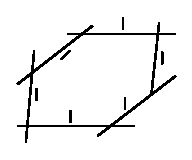
\includegraphics{vol37-figures/fig37-2(1).eps}}
\end{tabular}
\begin{tabular}{>{\raggedright}p{3cm}}
{($m$ components,  $m$ arbitrary $\rangle$ 1)}  
\end{tabular}

\medskip

  $G$ is an extension of $ \mathbb{Z}_{/_{m \mathbb {Z} }}$  by the
  multiplicative group $K^*$. 
\end{case*}

\begin{case*}[$(C ~1)$ ]~

\begin{minipage}{4cm}
  \begin{figure}[H]
    \centering{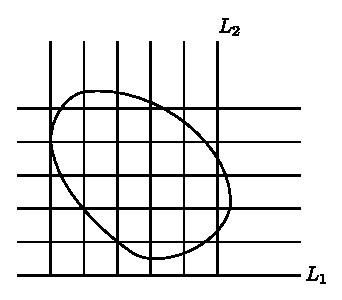
\includegraphics{vol37-figures/fig37-3.eps}}
  \end{figure}
\end{minipage}\qquad 
\begin{minipage}{4cm}
 $G$ is the additive group $K$.
\end{minipage}
\end{case*}

\begin{case*}[$(C ~2)$ ]~

\begin{minipage}{4cm}
  \begin{figure}[H]
    \centering{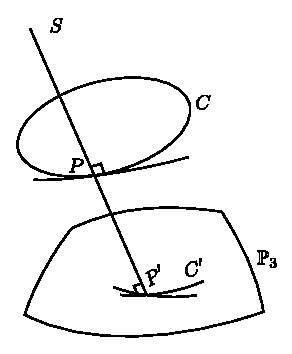
\includegraphics{vol37-figures/fig37-4.eps}}
  \end{figure}
\end{minipage}\qquad 
\begin{minipage}{4cm}
   $G$ is an extension of $\mathbb {Z}_{/_{2
      \mathbb {Z}}} $ by $K$ 
\end{minipage}
\end{case*}

\begin{case*}[$(C~ 3)$ ]~ 

\begin{minipage}{4cm}
  \begin{figure}[H]
    \centering{\includegraphics{vol37-figures/fig37-5.eps}}
  \end{figure}
\end{minipage}\qquad 
\begin{minipage}{4cm}
 $G$ is an extension of $\mathbb {Z}_{/_{3
      \mathbb {Z}}} $ by $K$ 
\end{minipage}
\end{case*}

\begin{case*}[$(C ~4)$ ]~ \pageoriginale

\begin{minipage}{4cm}
  \begin{figure}[H]
    \centering{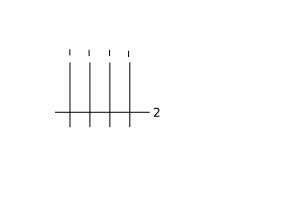
\includegraphics{vol37-figures/fig37-6.eps}}
  \end{figure}
\end{minipage}\qquad 
\begin{minipage}{4cm}
  $G$ is an extension of the Klein group
  $\mathbb {Z}_{/_{2 \mathbb {Z}}}  x   \mathbb {Z}_{/_{2 \mathbb
      {Z}}}$ by $K$ 
\end{minipage}
\end{case*}

\begin{case*}[$(C ~5_m)$ ]~

  \begin{figure}[H]
    \centering{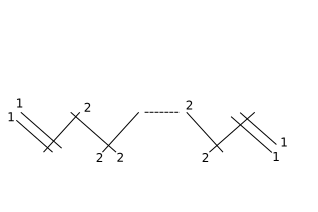
\includegraphics{vol37-figures/fig37-7.eps}}
  \end{figure}

  ($m+1$ components occurring with multiplicity $2$). $G$ is an
  extension of $\mathbb{Z}/4 \mathbb{Z}$ when $m$ is odd
  (\resp the Klein group when $m$ is even) by $K$. 
\end{case*}

\begin{case*}[$(C ~6)$ ]~ 

\begin{minipage}{5cm}
  \begin{figure}[H]
    \centering{\includegraphics{vol37-figures/fig37-8.eps}}
  \end{figure}
\end{minipage}\qquad 
\begin{minipage}{4.3cm}
  $G$ is an extension of $ \mathbb {Z}_{/_{3 \mathbb {Z}}}$ by $K$.
\end{minipage}
\end{case*}

\begin{case*}[$(C ~7)$ ]~ 

\begin{minipage}{5cm}
  \begin{figure}[H]
    \centering{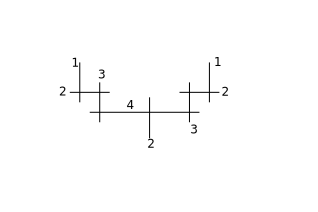
\includegraphics{vol37-figures/fig37-9.eps}}
  \end{figure}
\end{minipage}\qquad 
\begin{minipage}{4.3cm}
  $G $ is an extension of $ \mathbb {Z}_{/_{2 \mathbb {Z}}}$ by $K$.
\end{minipage}
\end{case*}

\eject

\begin{case*}[$(C ~8)$ ]~
\smallskip

\noindent
\begin{tabular}{l}
{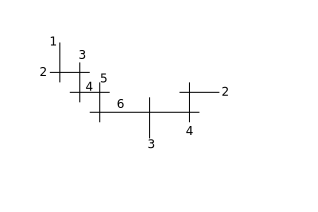
\includegraphics{vol37-figures/fig37-10.eps}}
\end{tabular}
\begin{tabular}[m]{l}
$G$ is isomorphic to $K$.
\end{tabular}


  This completes the list.	
\end{case*}

This\pageoriginale description of all degenerate fibres was given by
Kodaira in the 
geometric case and by Neron in the case $B=$ Spec $\mathscr O ,
\mathscr O$ a valuation ring with an algebraically  closed residue
field. Their proofs are quite different. Neron starts with  a model
$X'$ of $X$ which is a subscheme of $ \mathbb {P}^2 (\mathscr O)$ and
which corresponds to the Weierstrass normal for of the generic fibre
of $X$ over $R(B)$. This model is in general not regular.  

Resolving the  singularities by means of dilatations, N\'eron arrives at
the minimal model. This procedure is based on a detailed consideration of
many different particular cases. 

The proof of Kodaira is much easier. It is based on the consideration
of the intersection multiplicities of the components of degenerate
fibres and on formula (\ref{chap7:eq2}) of lecture \ref{chap7}. It
seems interesting to 
try to extend this proof to the  general case considered by Neron
-especially because such a proof has to be based on the consideration
of some generalisation of the canonical class $K$ to arbitrary
schemes. This is not the only question for which it seems essential
to have some notions corresponding to those of a canonical
class.tangent bundle etc. in the case of arbitrary two dimensional
schemes. For instance, one has the notion of a tangent plane at a
point $x$ (if $X$ is regular at  $x$) but  can one introduce some
structure in the totality  of all such planes? The absence of such
notions seems to be the principal hurdle if one tries to carry over
Grauert's proof (Publications Mathematiques $No.25, 131-149)$of
Manin's theorem to the case of a number field. 

\begin{thebibliography}{99}
\bibitem{key1} {S. Abhyankar}:\pageoriginale Ramification theoretic methods in
  algebraic geometry, Ann. of Math.Studies, N. 43, Princetion 1959 

\bibitem{key2} Algebraic Surfaces, Trudi Mat. Inst. Steklov, 75,
  Moscow (1965). by I.R Shafarevich et all 

\bibitem{key3} {G. Castelnuovo}: {Sulle superficie di genere
  zero. memsoc. It. delle Scienze (3) 10 (1896).}
 
\bibitem{key4} {F. Enriques}: {Sulle irazionalita da cui puo farsi
  dipendere la risoluzione d'un' equazione algebraica $f(x,y,z)=0$
  con funzioni razionali di due parametri, Math. Ann. 49 (1897)} 

\bibitem{key5} {H. Grauert}: {\"Uber Modifikationen und exzebtionelle
  analytische Menagen. Math. Ann. 146 (1962).} 

\bibitem{key6} {M.  Greenberg}: {Schemata over local rings. Ann. of
  Math. (2) 73 (1961).} 

\bibitem{key7} {A. Grothendicek}: {Elements de geometrie algebrique
  $(E.G.A)$ Publications Mathematiques de l'Institut des Hautes Etudes
  Scientifiques.} 

\bibitem{key8} {A. Grothendieck}: {Fondements de la Geometrie Algebrique.Paris
  $1962$} 

\bibitem{key9} {A. Grothendieck}:\pageoriginale {Seminaire de
  Geometrie Algebrique,   $(S.G.A)$, Institut des Hautes Etudes
  Scientifiques, Paris 1960.}  

\bibitem{key10} {H. Hasse}: {Aquivalenz quadratischer Formen in einem
  beliebigen algebraischen Zahlkorper, Journ. fur die Reine und
  Angew. Math. 153. 1924.} 

\bibitem{key11} {H. Hironaka}: {Afundamental lemma on point
  modifications,  

  Proceedings of the conference on complex analysis, Springer 1965.}

\bibitem{key12} {W. Hodge and  D. Pedoe}: { Methods of algebraic geometry,
  $II$. Cambridge 1952.} 

\bibitem{key13} {K. Kodaira}: {On compact complex analytic
  surfaces. $II$. Ann. of Math. 77 (1963).} 

\bibitem{key14} {S. Lang}: {Introduction to algebraic geometry, Interscience 1958.}

\bibitem{key15} {S. Lang}: {Abelian Varieties, Interscience, 1959.}

\bibitem{key16} {S. Lang and A. Neron}: {Rational points of abelian varieties
  over function fields, Amer. Journ. of Math.  81 (1959).} 

\bibitem{key17} {D. Mumford}: {The topology of normal singularities of  and
  algebraic surface and a criterion for simplicity, Publications
  Mathematiques de l'Institut des Haut es Etudes Scientifiques,
  9. 1961.} 

\bibitem{key18} {Nagata}:\pageoriginale {On rational surfaces $I$;
  Memoirs of the  College 
  of Science, University of Tokyo, Series A, 32 (1960).} 

\bibitem{key19} {M. Nagata}: {Imbedding of an abstract variety in a complete
  variety, Journ. Math. Kyoto Univ. 2 (1962).} 

\bibitem{key20} {A. Neron}: {Modelesminimaux, Publications Mathematiques de
  l'Institut des Hautes Etudes Scientifiques. No 21} 

\bibitem{key21} {J.P. Serre}: {Cohomologie Galoisienne, Lecture Notes in
  Mathematics, 5, Springer, 1964.} 

\bibitem{key22} {A. Weil}: {Sur les criteres d'equivalence en geometrie
  algebrique Math. Ann. 128 (1954).} 

\bibitem{key23} {O. Zariski}: {Introduction to the problem of minimal
  models in   the theory of algebraic surfaces, Tokyo Math.Soc. of
  Japan 1958.}  

\bibitem{key24} {O. Zariski}: {The problem of minimal models in the theory of
  algebraic surfaces, Amer. journ.of Math. 80(1958).} 

\bibitem{key25} {O. Zariski}: {On Castelnuovo's criterion of rationality of
  an algebraic surface, Illinois Journ. of Math. 2 (1958).} 

\bibitem{key26} {O. Zariski and P.Samuel.}: {Commutative Algebra, $V$. $II$
  van Nostrand. } 

\bibitem{key27} {O. Zariski}: {Algebraic sheaf theory,
  Bull. Amer. Math. soc. 62 (1956).} 

\bibitem{key28} {C. Chevalley}:\pageoriginale {Fondements de la geometie algebrique
  (Fondements), Paris 1958.} 

\bibitem{key29} {M. Nagata}: {Local rings (L.R) Inter Science
  Publishers, New   York.} 

\bibitem{key30} {R. Godement}: {Topologie algebrique et theorie des faisceux,
  Hermann et cie, Paris.} 

\bibitem{key31} {Seminaire C.}: {Chevalley,Anneaux de Chow et ses
  applications. (Anneux de Chow)} 

\bibitem{key32}{S. Lang}: {Diophantine Geometry (Dioph. Geom.) Inter Science
  Publishers, New York.} 

\bibitem{key33} {G. Castelnovo}: {Sulla razionalita delle involuzioni pinne
  Math. Ann. 44 (1894)  P.125-155.} 

\bibitem{key34} {J.P. Serre}: {Critere de rationalite pour les surfaces
  algebriques (d'apres un cours de K.Kodaira)Seminaire
  Bourbaki,Fevrier 1957.} 

\bibitem{key35} {J.P. Serre}: {Corps Locaux, Paris, 1962.} 

\bibitem{key36} {T. Matsusaka}: {The criteria for algebraie equivalence and
  the torsion group. Amer. J. of Maths. Vol. 79 (1957) P.53-66.} 

\bibitem{key37} {F. Enriques}: {Sulle superficie algebriche di
  generegeometrico zero. Rendic Circ. Palermo 20  (1905) p.1.} 
\end{thebibliography}

